\documentclass{article}

\usepackage{graphicx}
\begin{document}

The roots of Ukrainian national symbols come from pre-Christian times when yellow and blue prevailed in traditional ceremonies, reflecting fire and water. During the battle of Grunwald in 1410 two Polish banners of Lwow and Przemysl Lands used flags with yellow and blue colours.

Blue-yellow, red-black, crimson-olive and especially raspberry colour banners were widely used by Cossacks between the 16th and 18th centuries. These were not the only possible combinations, since normally Cossacks would fly their hetman's banners, which were similar to the coats of arms of the nobility. Also, yellow and blue were the colours common on coats of arms in Galicia. In fact, the coat of arms of Lviv to this day remains a golden lion on a blue field.

Some put the starting point of the adoption of the current national flag of Ukraine to 1848 when, during the Spring of the Nations on 22 April 1848, a blue-and-yellow banner was adopted by the Supreme Ruthenian Councilin Lemberg (Lviv), the capital of the Kingdom of Galicia and Lodomeria, and flew over the city's magistrate for the first time. Although this move did not have significant consequences, the newly formed Ukrainian divisions in the Austrian army used blue-and-yellow banners in their insignia.

\begin{center}
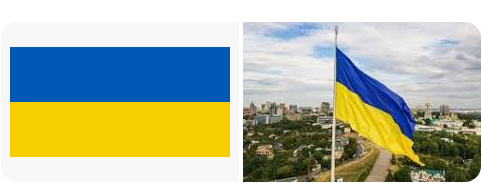
\includegraphics [width=345pt,keepaspectratio]{зображення_2022-12-10_195419904.png}
\end{center}


\end{document}
